	%Version 3 October 2023
% See section 11 of the User Manual for version history
%
%%%%%%%%%%%%%%%%%%%%%%%%%%%%%%%%%%%%%%%%%%%%%%%%%%%%%%%%%%%%%%%%%%%%%%
%%                                                                 %%
%% Please do not use \input{...} to include other tex files.       %%
%% Submit your LaTeX manuscript as one .tex document.              %%
%%                                                                 %%
%% All additional figures and files should be attached             %%
%% separately and not embedded in the \TeX\ document itself.       %%
%%                                                                 %%
%%%%%%%%%%%%%%%%%%%%%%%%%%%%%%%%%%%%%%%%%%%%%%%%%%%%%%%%%%%%%%%%%%%%%
%%\documentclass[referee,sn-basic]{sn-jnl}% referee option is meant for double line spacing

%%=======================================================%%
%% to print line numbers in the margin use lineno option %%
%%=======================================================%%

%%\documentclass[lineno,sn-basic]{sn-jnl}% Basic Springer Nature Reference Style/Chemistry Reference Style

%%======================================================%%
%% to compile with pdflatex/xelatex use pdflatex option %%
%%======================================================%%

%%\documentclass[pdflatex,sn-basic]{sn-jnl}% Basic Springer Nature Reference Style/Chemistry Reference Style


%%Note: the following reference styles support Namedate and Numbered referencing. By default the style follows the most common style. To switch between the options you can add or remove �Numbered� in the optional parenthesis. 
%%The option is available for: sn-basic.bst, sn-vancouver.bst, sn-chicago.bst%  
 
%%\documentclass[sn-nature]{sn-jnl}% Style for submissions to Nature Portfolio journals
%%\documentclass[sn-basic]{sn-jnl}% Basic Springer Nature Reference Style/Chemistry Reference Style
\documentclass[sn-mathphys-num]{sn-jnl}% Math and Physical Sciences Numbered Reference Style 
%%\documentclass[sn-mathphys-ay]{sn-jnl}% Math and Physical Sciences Author Year Reference Style
%%\documentclass[sn-aps]{sn-jnl}% American Physical Society (APS) Reference Style
%%\documentclass[sn-vancouver,Numbered]{sn-jnl}% Vancouver Reference Style
%%\documentclass[sn-apa]{sn-jnl}% APA Reference Style 
%%\documentclass[sn-chicago]{sn-jnl}% Chicago-based Humanities Reference Style

%%%% Standard Packages
%%<additional latex packages if required can be included here>

\usepackage{graphicx}%
\usepackage{multirow}%
\usepackage{amsmath,amssymb,amsfonts}%
\usepackage{amsthm}%
\usepackage{mathrsfs}%
\usepackage[title]{appendix}%
\usepackage{xcolor}%
\usepackage{textcomp}%
\usepackage{manyfoot}%
\usepackage{booktabs}%
\usepackage{algorithm}%
\usepackage{algorithmicx}%
\usepackage{algpseudocode}%
\usepackage{listings}%


%%%%

%%%%%=============================================================================%%%%
%%%%  Remarks: This template is provided to aid authors with the preparation
%%%%  of original research articles intended for submission to journals published 
%%%%  by Springer Nature. The guidance has been prepared in partnership with 
%%%%  production teams to conform to Springer Nature technical requirements. 
%%%%  Editorial and presentation requirements differ among journal portfolios and 
%%%%  research disciplines. You may find sections in this template are irrelevant 
%%%%  to your work and are empowered to omit any such section if allowed by the 
%%%%  journal you intend to submit to. The submission guidelines and policies 
%%%%  of the journal take precedence. A detailed User Manual is available in the 
%%%%  template package for technical guidance.
%%%%%=============================================================================%%%%

%% as per the requirement new theorem styles can be included as shown below
\theoremstyle{thmstyleone}%
\newtheorem{theorem}{Theorem}%  meant for continuous numbers
%%\newtheorem{theorem}{Theorem}[section]% meant for sectionwise numbers
%% optional argument [theorem] produces theorem numbering sequence instead of independent numbers for Proposition
\newtheorem{proposition}[theorem]{Proposition}% 
%%\newtheorem{proposition}{Proposition}% to get separate numbers for theorem and proposition etc.

\theoremstyle{thmstyletwo}%
\newtheorem{example}{Example}%
\newtheorem{remark}{Remark}%

\theoremstyle{thmstylethree}%
\newtheorem{definition}{Definition}%

\raggedbottom
%%\unnumbered% uncomment this for unnumbered level heads

\begin{document}

\title[Article Title]{Beyond Static Retrieval: Adaptive Method for Improving RAG Performance}

%%=============================================================%%
%% GivenName	-> \fnm{Joergen W.}
%% Particle	-> \spfx{van der} -> surname prefix
%% FamilyName	-> \sur{Ploeg}
%% Suffix	-> \sfx{IV}
%% \author*[1,2]{\fnm{Joergen W.} \spfx{van der} \sur{Ploeg} 
%%  \sfx{IV}}\email{iauthor@gmail.com}
%%=============================================================%%

\author*[1]{\fnm{Zoubida Asmaa} \sur{Boudjenane }}\email{asmaa.boudj04@gmail.com}

\author[2]{\fnm{Mohammed} \sur{Salem}}\email{salem@univ-mascara.dz}
\equalcont{These authors contributed equally to this work.}

%\author[1,2]{\fnm{Third} \sur{Author}}\email{iiiauthor@gmail.com}
%\equalcont{These authors contributed equally to this work.}

\affil*[1]{\orgdiv{Computer Science Department}, \orgname{University of Mascara}, \orgaddress{\street{Street}, \city{Mascara}, \postcode{29000}, \state{}, \country{Algeria}}}

\affil*[2]{\orgdiv{LISYS Lab}, \orgname{University of Mascara}, \orgaddress{\street{Street}, \city{City}, \postcode{100190}, \state{State}, \country{Algeria}}}

%\affil[3]{\orgdiv{Department}, \orgname{Organization}, \orgaddress{\street{Street}, \city{City}, \postcode{610101}, \state{State}, \country{Country}}}

%%==================================%%
%% Sample for unstructured abstract %%
%%==================================%%

\abstract{Retrieval-Augmented Generation (RAG) improves the quality of language model responses by incorporating external knowledge. However, its performance heavily relies on choosing the right number of documents to retrieve (K). Using a fixed number of documents (K) is computationally efficient but fails to adapt to the complexity of different queries. On the other hand, dynamically adjusting K offers flexibility but comes with higher computational costs and inconsistency. To overcome these challenges, we introduce a hybrid approach to dynamic K selection. This method adapts K based on the specific characteristics of each query while keeping computational demands manageable. Our strategy enhances retrieval performance by minimizing irrelevant information, ensuring the retrieval of relevant data, and boosting overall system accuracy. Experiments show that this approach outperforms both fixed and fully dynamic methods, offering a promising way to optimize retrieval in RAG systems.Future research will focus on developing learning-based techniques to further improve the dynamic selection of K.}

%%\pacs[JEL Classification]{D8, H51}

%%\pacs[MSC Classification]{35A01, 65L10, 65L12, 65L20, 65L70}

\maketitle

\section{Introduction}\label{sec1}

Large Language Models (LLMs)\cite{Radford2019} have emerged as state-of-the-art artificial intelligence systems that excel at understanding and generating human-like text,Built on deep learning architectures,particularly transformers \cite{vaswani2017attention}.these models are trained on massive datasets to capture linguistic patterns and semantic relationships showcasing impressive adaptability across diverse tasks such as  machine translation\cite{Gu2018SearchEngine}, text generation\cite{liang2024controllabletextgenerationlarge} and question answering\cite{Zhang2023}.Notable examples of LLMs include OpenAI GPT series\cite{brown2020language} , Google BERT\cite{devlin2018bert} and T5 \cite{raffel2020exploring} which have set new benchmarks in NLP tasks .\\
Despite their impressive capabilities,LLMs suffer from hallucination\cite{ji2023survey} where they confidently generate factually incorrect or entirely fabricated information. This poses challenges in applications requiring high accuracy like knowledge-intensive tasks\cite{kandpal2023large} , Additionally significant limitation of LLMs is their static nature, as they are trained on fixed datasets\cite{bender2021dangers} and cannot dynamically update their knowledge which makes them prone to generating outdated or inconsistent responses, especially for time-sensitive or evolving data\cite{Mousavi2025}. 


Researchers have explored various approaches To address this limitation, including transfer learning\cite{zhuang2020comprehensive}a technique that improves pre-trained models performance in new tasks by transferring knowledge from related tasks.and fine-tuning \cite{Howard2018} which adapt pre-trained models to specific tasks or domains. While these methods improve performance on targeted tasks,they are computationally expensive and impractical for real-time knowledge updates. A promising alternative is Retrieval-Augmented Generation (RAG) \cite{lewis2020retrieval}.which integrates real-time retrieval from external knowledge sources with generative models.

RAG enables LLMs to access up-to-date information without retraining, making it particularly useful for applications like open-domain question answering and fact-checking.
Retrieval-Augmented Generation (RAG) faces several limitations, The performance of RAG heavily depends on the quality of the retriever \cite{karpukhin2020dpr}, as irrelevant or noisy documents can degrade the generator output. Additionally, retrieving and processing a large number of documents increases computational overhead , making RAG less efficient for real-time applications. A critical challenge is determining the optimal number of retrieved passages (K) to feed into the generator\cite{lewis2020retrieval}. often resulting in either insufficient or excessive information being retrieved, reduce coherence and increase computational overhead. This trade-off makes K a key factor in balancing performance and efficiency. 

Current approaches, such as static K selection \cite{lewis2020retrieval} involves retrieving a fixed number of top results regardless of the query characteristics ,it cannot adapt to the complexity of individual queries , dynamic K adjustment attempt to address this trade-off but often introduce complexity or latency ,Hybrid approaches like those proposed yuan et al . \cite{yuan2024hybrid},that integrates static retrieval with dynamic retrieval to improve accuracy. Furthermore, the "Blended RAG"\cite{sawarkar2024blendedragimprovingrag} approach \cite{blended_rag2024} enhances retrieval accuracy by combining semantic search techniques with hybrid query strategies. However, the approach faces significant limitations, including high computational overhead due to the need for multiple retrieval methods and dependency on high-quality metadata for optimal performance. These limitations highlight the need for a more robust approach to K selection, capable of balancing efficiency and accuracy across varying query types.


In this paper, we investigate the problem of selecting K in RAG and propose a novel approach to dynamically adjust K based on  thresholds and a Mixture of Logits (MoL)\cite{ding2024efficient} scoring mechanism, ensuring efficient and context-sensitive candidate selection while reducing computational costs. the use of  adaptive thresholds algorithm improves the relevance of retrieved documents, refining the set to include only the most contextually appropriate matches. Unlike traditional approaches, it adapts to the query and dataset characteristics, making it more flexible for diverse contexts. Furthermore, its design for handling large datasets ensures scalable and precise retrieval, which is crucial for RAG systems working with extensive corpora.

Our contributions in this paper are the following :
we review existing approaches to Retrieval-Augmented Generation (RAG), with a specific focus on static , dynamic and Hybrid selection strategies. We critically analyze the strengths and limitations of these methods, identifying key gaps in their design and performance. These gaps motivate the need for an improved approach that addresses the challenges of both static and dynamic in retrieval-augmented systems. \\
Overview of Retrieval-Augmented Generation (RAG) in This section We provide a detailed explanation of the RAG framework, including its components and how it operates. Key concepts, such as retrievers, generators are discussed to establish the foundational context.\\
Proposed Solution: This section introduces our novel hybrid dynamic  selection algorithm. We describe its methodology, explain its design, and discuss how it overcomes the limitations of existing static and dynamic approaches. The benefits of this approach, particularly in improving retrieval accuracy and computational efficiency, are emphasized.\\
Results :in This section We present experimental results to demonstrate the effectiveness of our hybrid dynamic  selection algorithm. Comparisons with baseline method highlight its superiority in terms of retrieval performance and adaptability to diverse query complexities.


\section{Related works}\label{sec2}
The selection of an optimal number of retrieved items (K) in Retrieval-Augmented Generation (RAG) systems plays a crucial role in ensuring accurate and efficient responses.Several methods, including static, dynamic, and hybrid approaches have been proposed to address this challenge While these methods show promise in improving performance,they often face trade-offs between adaptability, efficiency when applied to complex or diverse query patterns. In this section, we will explore these methods, highlight their respective strengths and weaknesses, and introduce our hybrid solution as a more robust and adaptable alternative. \\
\textbf{Static Top-K selection in Retrieval} 


In traditional Retrieval-Augmented Generation (RAG) systems, static K-selection is a widely used method where a fixed number of top-k documents are retrieved based on their relevance scores. Sparse retrieval methods where the "keys" represent documents to be retrieved, and the "values" are the same documents in this context such as query likelihood models\cite{Lafferty2001} ,TF-IDF\cite{Robertson1997} and BM25\cite{Zaragoza2009} often rely on this static approach to identify and rank documents. For instance, if k  =5, the system retrieves the top 5 documents deemed most relevant to a query, regardless of the query's complexity or the variability in relevance distribution among documents.
A major drawback of this approach is its rigidity. Since the number of retrieved documents (k) is fixed, it fails to adapt to the varying complexity of queries. For simple queries, retrieving too many documents may introduce noise, while for complex queries, retrieving too few may result in incomplete or insufficient information. This one-size-fits-all strategy can lead to suboptimal performance across diverse datasets or tasks.\\
\textbf{Dynamic top-k Selection in Retrieval}

Dynamic k-selection addresses the limitations of static k by varying the number of retrieved documents based on the specific query or context. These approaches typically involve heuristics, machine learning models, or adaptive algorithms to determine the optimal K for each query such as Dynamic Query Cutoff (DQC)\cite{Culpepper2016} This approach uses machine learning models trained on query-document features to predict the optimal k for retrieval , A reinforcement learning-based approach\cite{Zhou2021} where the agent learns to adjust k by maximizing downstream task performance (e.g accurate response generation in RAG) Another example is the Dynamic Selection of k Nearest Neighbors \cite{DynamicKNN2012} where the selection process often depends on the distribution of neighbors, their distances to the query point, or their relevance scores.
However, these methods come with limitations.They often introduce computational overhead due to the need for dynamic evaluation, which can increase latency in large-scale systems. Additionally, their performance heavily depends on the quality of the underlying models or distance metrics, making them sensitive to noisy data or poorly tuned hyperparameters. As a result, achieving generalization across diverse datasets or domains remains a significant challenge. \\
\textbf{Hybrid Approaches}

Hybrid approaches combine elements of static and dynamic K-selection to achieve a balance between simplicity and adaptability.These systems might use a static 
k as a baseline but dynamically adjust such as STAYKATE (Static-Dynamic Hybrid Selection)\cite{Zhu2024} Combines static (active learning-inspired) and dynamic (KATE-based) example selection strategies to create STAYKATE. Another example is DR-RAG (Dynamic Relevance for Retrieval-Augmented Generation)\cite{hei2024drragapplyingdynamicdocument} retrieval framework designed to improve the relevance between queries and documents. In the first stage, a similarity matching method retrieves an initial set of documents. In the second stage, a deeper analysis is performed to identify dynamic-relevant documents, supported by a classifier that filters out irrelevant ones . however hybrid methods may face challenges in determining when to apply static or dynamic k-selection effectively, leading to potential trade-offs between retrieval accuracy and system efficiency. These limitations highlight the ongoing need for robust mechanisms that dynamically and efficiently adapt k to the unique characteristics of each query and dataset.

Our method leverages adaptive thresholds to dynamically refine the list of retrieved documents, to make sure that only the most contextually relevant matches are included. In contrast to traditional static or fixed K-selection techniques, which employ a consistent retrieval strategy for every query, our approach adapts to the specific characteristics of both the query and the dataset. This flexibility allows the algorithm to better accommodate diverse contexts, enhancing the relevance and quality of retrieval results.Through its adaptive nature, the method not only improves retrieval accuracy but also minimizes computational overhead by focusing resources on the most pertinent results. 

\section{Overview of Retrieval-Augmented Generation }\label{sec3}
Retrieval-Augmented Generation (RAG) is a method designed to enhance the performance of large language models (LLMs) by integrating external, reliable knowledge sources into their response generation process\cite{awsRAG}. RAG combines search capabilities with LLM prompting. The process involves feeding both the userss query and the relevant information retrieved by a search algorithm into the LLMs prompt\cite{ilin2023advancedrag}, enabling the model to generate answers based on the provided context.

\begin{figure}[h]
	\centering
	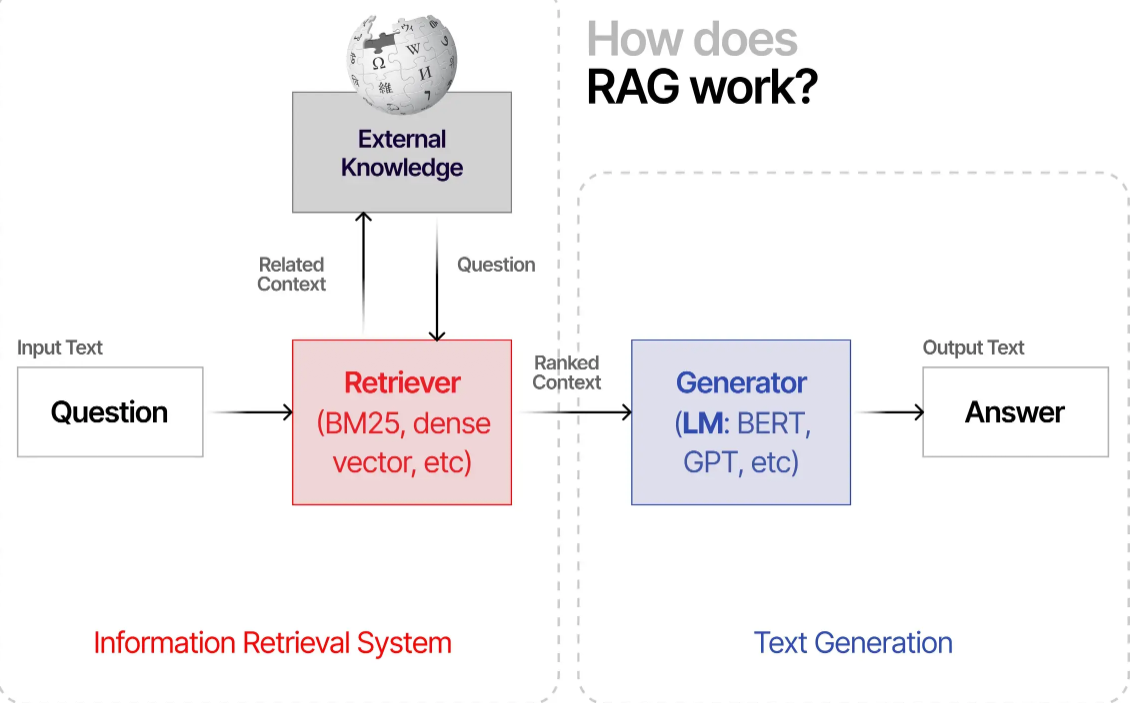
\includegraphics[width=0.9\textwidth]{rag.PNG}
	\caption{RAG system component }\label{rag.PNG}
\end{figure}
As illustrated in figure \ref{rag.PNG}, the RAG system is built around two main components:the retriever and the generator. The retriever?s role is to find relevant information from a pre-built data store, while the generator utilizes this retrieved data to produce coherent and contextually appropriate content. The overall RAG process operates as follows:
\subsection{Retrieval in RAG Systems}\label{subsec2}

Retrieval is the process of identifying and gathering information system resources that match a specific information need. To break it down, imagine these resources as a key-value store, represented as pairs:

\[
\{(k_i, v_i)\}_{i=1}^{N}
\]

where each key \( k_i \) is linked to a corresponding value \( v_i \) (often, the key and value are the same). When a query \( q \) is provided, the goal is to find the top-\( k \) keys that are most similar to the query using a similarity function \( s \), and then retrieve their associated values\cite{gupta2024comprehensivesurveyretrievalaugmentedgeneration}.

Depending on the similarity function used, retrieval methods can be grouped into categories such as sparse retrieval, dense retrieval, and others. For the widely used sparse and dense retrieval approaches, the process typically involves two main steps:  \\
1. Encoding each object into a specific representation.\\
2. Building an index to organize the data for efficient searching .

This structured approach ensures that the most relevant information is retrieved quickly and accurately\cite{zhao2024retrievalaugmentedgenerationaigeneratedcontent}.

\subsection{Generator  in RAG Systems}\label{subsec2}
In Retrieval-Augmented Generation (RAG) systems, the generator is a key component responsible for crafting the final output. It works by combining the retrieved information with the users input query to produce a well-structured and contextually relevant response .

Once the retriever fetches relevant data from external sources,the generator processes and integrates this information into a well-structured and meaningful answer. At the core of this process is a Large Language Model (LLM), which ensures that the generated text is not only fluent and accurate but also remains relevant to the original query.

In various generative tasks, different models are selected based on the specific requirements: Models like BART\cite{lewis2019bart} and GPT\cite{brown2020language}are commonly used for tasks such as text summarization and translation ,Vision-Language Models (VLMs) \cite{radford2021learningtransferablevisualmodels} are employed to generate textual descriptions from images , for ext-to-Code Generation: Models like OpenAIs Codex \cite{chen2021evaluatinglargelanguagemodels} are designed to translate natural language prompts into executable code.


\section{proposed Slution}\label{sec3}
In traditional candidate selection systems, the reliance on static or fixed top-K retrieval lead to suboptimal retrieval performance, especially in scenarios where the relevance distribution of candidates is highly variable. To address these limitations, we propose Dynamic Candidate Selection, a novel algorithm that adaptively refines the candidate selection process by leveraging component-level embeddings and a Mixture of Logits (MoL) scoring mechanism.


The \textbf{Mixture of Logits (MoL)}\cite{zhai2023revisiting} methode provides a flexible and adaptive mechanism for computing similarity scores between queries and items. Given a query \( q \) and an item \( x \), MoL assumes that both are mapped to \( P \) groups of low-rank embeddings, denoted as \( f_p(q) \) and \( g_p(x) \), respectively. These embeddings are parameterized by neural networks that extract features from the query and item. The similarity between \( q \) and \( x \) is computed as a weighted sum of the inner products of these embeddings, where the weights \( \pi_p(q, x) \)\cite{zhai2023revisiting} are adaptive gating parameters constrained to sum to 1:
\[
\text{Similarity}(q, x) = \sum_{p=1}^P \pi_p(q, x) \cdot \langle f_p(q), g_p(x) \rangle.
\]
This formulation allows MoL to capture complex relationships between queries and items, making it particularly suitable for dynamic candidate selection tasks.


Inspired by the approach in\cite{ding2024efficient}, we introduce an adaptive threshold mechanism (\textbf{Dynamic Candidate Selection}), the MoL framework is employed to refine the candidate retrieval process. Specifically:
\begin{enumerate}
	\item \textbf{Component-Level Embeddings:}  
	 generate component-level embeddings for all items in \( X \). These embeddings allow efficient similarity computations during retrieval.
	\begin{equation*}
		X_p \leftarrow \{ g_p(x) \mid x \in X \}
	\end{equation*}
	
	\item \textbf{Dynamic Threshold Adjustment:}  
	To refine retrieval quality, we compute Mixture of Logits (MoL) scores for each candidate \( x \in G \).  
	The adaptive gating weights \( \pi_p(q, x) \) enable the algorithm to dynamically adjust the retrieval threshold \( T_{\text{adaptive}} \) based on the computed MoL scores.
	\begin{equation*}
		\varphi(q, x) = \sum_{p=1}^{P} \pi_p(q, x) \cdot \langle f_p(q), g_p(x) \rangle
	\end{equation*}
	\begin{equation*}
		T_{\text{adaptive}} = \min \{ s \mid s \in G \}
	\end{equation*}
	
	\item \textbf{Refinement and Top-K Selection:}  
	Additional relevant candidates are retrieved using the adaptive threshold \( T_{\text{adaptive}} \), expanding the candidate set \( G' \). The algorithm then selects the most relevant top-k results by sorting \( G' \) based on MoL scores.
	\begin{equation*}
		G' \leftarrow G \cup \{ x \mid s_p \geq T_{\text{adaptive}} \}
	\end{equation*}
	Finally, we sort candidates by MoL scores and extract the exact top-k:
	\begin{equation*}
		G_{\text{final}} = \text{Top-}k(G', \varphi(q, x))
	\end{equation*}
\end{enumerate}
the flowchart provided in Figure~\ref{fig2} describes the step-by-step process of the proposed algorithm. It visualizes the key stages of the solution
\begin{figure}[H]
	\centering
	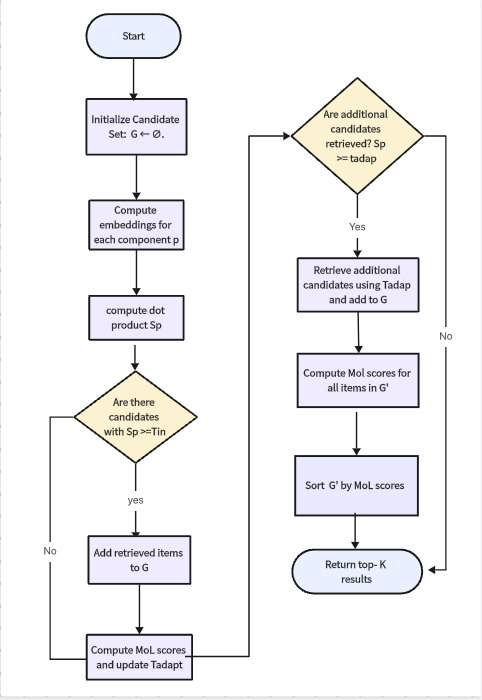
\includegraphics[width=0.9\textwidth]{Flowchart_Steps.PNG}
	\caption{Algorithm workflow. }\label{fig2}
\end{figure}


As shown in Algorithm~\ref{Algo1}, the retrieval process dynamically adjusts the threshold based on MoL scores.
\begin{algorithm}
	\caption{Hybrid Exact Top-k with Threshold-Based k Selection}\label{ALgo1}
	\begin{algorithmic}[1]
		\State \textbf{Input:}
		\begin{itemize}
			\item Query $q$
			\item Set of items $X$
			\item Component-level embeddings: $f_p(q)$, $g_p(x)$ for $p \in P$, $x \in X$
			\item Initial threshold $T_{\text{init}}$
		\end{itemize}
		
		\State \textbf{Output:}
		\begin{itemize}
			\item Exact top $k$ items based on dynamic threshold selection, $G_{\text{final}}$
		\end{itemize}
		
		\State \textbf{1. Initialize:}
		\begin{itemize}
			\item Set $G \gets \emptyset$ \Comment{Initial candidate set}
		\end{itemize}
		
		\State \textbf{2. Generate Component-Level Embeddings:}
		\For{each component $p \in P$}
		\State $X_p \gets \{g_p(x) \mid x \in X\}$ \Comment{Precompute embeddings}
		\EndFor
		
		\State \textbf{3. Initial Candidate Retrieval:}
		\For{each component $p \in P$}
		\State Compute dot product scores: 
		\[
		S_p = \{ \langle f_p(q), g_p(x) \rangle : x \in X_p \}
		\]
		\State Retrieve items with scores $S_p \geq T_{\text{init}}$
		\State Add these items to $G$
		\EndFor
		
		\State \textbf{4. Adjust k Dynamically:}
		\For{each $x \in G$}
		\State Compute MoL scores $s = \phi(q, x)$ for each $x \in G$ using:
		\[
		\phi(q, x) = \sum_{p=1}^{P} \pi_p(q, x) \cdot \langle f_p(q), g_p(x) \rangle
		\]
		\State Set $T_{\text{adaptive}} = \min \{s : s \in G\}$
		\EndFor
		
		\State \textbf{5. Refine Candidate Set with Adaptive k:}
		\For{each component $p \in P$}
		\State Retrieve items from $X_p$ with scores $S_p \geq T_{\text{adaptive}}$
		\State Add these items to $G'$
		\EndFor
		
		\State \textbf{6. Select Exact Top-k Items:}
		\State Compute MoL scores for all items in $G'$
		\State Sort $G'$ by MoL scores in descending order
		\State Select the top $k$ items from $G'$ where $k$ is the number of items in $G'$ exceeding $T_{\text{adaptive}}$
		
		\State \textbf{7. Return:} $G_{\text{final}}$ \Comment{Top $k$ items from $G'$}
	\end{algorithmic}
\end{algorithm}
\section{Experimental Results}\label{sec3}
We evaluate the performance of our hybrid retrieval algorithm and the Mixture-of-Logits (MoL) approach on the next-item prediction task in recommendation systems\cite{Zhu_2018}\cite{kang2018selfattentivesequentialrecommendation}. We conducted experiments using two MovieLens datasets: ML-100K and ML-1M \cite{Harper2015}  which are widely used benchmarks for evaluating sequential recommendation models.\\
\textbf{MovieLens-100K} \\
100,000 ratings (1-5 scale) from 943 users on 1,682 movies\\
Each user has rated at least 20 movies \\
Includes user demographic information (age, gender, occupation, zip code)\\
\textbf{MovieLens-1M} \\
1,000,209 ratings from 6,040 users on approximately 3,900 movies \\
Data collected from users who joined MovieLens in 2000 \\
Represents a larger-scale recommendation scenario \\
\subsection{ Setup }
For both datasets, We utilize the SASRec architecture as our sequential user encoder, a model renowned for achieving state-of-the-art performance in next-item prediction tasks. This architecture processes the user's historical interaction sequence, generating embeddings that encapsulate the user's preferences at each time step. These embeddings serve as the foundation for predicting the next item in the sequence.\\

The query q represents the user's state at a specific time step, derived from their interaction history. In the MoL (Mixture of Logits) framework, q is transformed into Pq
embeddings through a multi-layer perceptron (MLP). While our hybrid algorithm does not explicitly employ an MLP for this transformation
\subsection{Hyperparameter settings.}
For fair comparison, we maintained consistent architectural choices and training conditions across all experiments , We conducted an extensive hyperparameter analysis comparing both approaches (Hybrid+SAS and MoL+SAS) across different architectural configurations.All experiments were pmplemented in TensorFlow and trained on a Google Colab environment with a T4 GPU. We use the Adam optimizer with a learning rate of 0.001. For the hybrid algorithm, we initialize the threshold (Tinit) to 0.3 and adaptively adjust it during training. .We discuss detailed
hyperparameter settings Table\ref{tab:100k_movies},table\ref{tab:1m_movies}
\begin{table}[h]
	\centering
	\resizebox{\textwidth}{!}{ % Scales the table to text width
		\begin{tabular}{lcccccccccc}
			\toprule
			Model & Max Seq Len & Embed Dim & Num Heads & FF Dim & Batch Size & Epochs & Val Loss & Val Accuracy \\
			\midrule
			Hybrid+SAS & 50  & 128  & 2 & 128  & 128 & 12 & 5.3036 & 0.1584  \\
			MoL+SAS    & 50  & 128  & 2 & 128  & 128 & 12 & 5.3152 & 0.1582  \\
			Hybrid+SAS & 128 & 256  & 4 & 256  & 128 & 10 & 3.6364 & 0.4301  \\
			MoL+SAS    & 128 & 256  & 4 & 256  & 128 & 10 & 3.6374 & 0.4299 \\
			Hybrid+SAS & 512 & 512  & 4 & 512  & 128 & 10 & 1.2808 & 0.8120 \\
			MoL+SAS    & 512 & 512  & 4 & 512  & 128 & 10 & 1.3050 & 0.8016 \\
			\bottomrule
		\end{tabular}
	}
	\caption{Results on 100kMovies dataset}
	\label{tab:100k_movies}
\end{table}

\begin{table}[h]
	\centering
	\resizebox{\textwidth}{!}{ 
		\begin{tabular}{lcccccccccc}
			\toprule
			Model & Max Seq Len & Embed Dim & Num Heads & FF Dim & Batch Size & Epochs & Val Loss & Val Accuracy  \\
			\midrule
			Hybrid+SAS & 50  & 128  & 2 & 128  & 128 & 10 & 4.5721 & 0.1530  \\
			MoL+SAS    & 50  & 128  & 2 & 128  & 128 & 10 & 4.5733 & 0.1526  \\
			Hybrid+SAS & 128 & 256  & 4 & 256  & 128 & 10 & 3.4152 & 0.3680  \\
			MoL+SAS    & 128 & 256  & 4 & 256  & 128 & 10 & 3.4671 & 0.3627  \\
			Hybrid+SAS & 512 & 512  & 4 & 512  & 128 & 10 & 1.0275 & 0.8350  \\
			MoL+SAS    & 512 & 512  & 4 & 512  & 128 & 10 & 1.0350 & 0.8276  \\
			\bottomrule
		\end{tabular}
	}
	\caption{Results on 1M Movies dataset}
	\label{tab:1m_movies}
\end{table}
\newpage
Both approaches demonstrate significant performance improvements as model capacity increases, with larger configurations consistently delivering better results. For instance, when increasing the model's capacity?such as expanding the (Max Sequence Length: 512, Embedding Dimension: 512, Number of Heads: 4, Feed-Forward Dimension: 512) the hybrid algorithm combined with SASRec (Hybrid+SAS) achieves notable gains, particularly in the most resource-intensive setup. On the ML-100K dataset, Hybrid+SAS reaches a score of\textbf{ 0.8120} compared to the baseline's \textbf{0.8016}, while on ML-1M, it achieves \textbf{0.8350} versus \textbf{0.8276.} The ML-1M dataset generally benefits more from increased capacity, with the performance gap between datasets narrowing as the model scales. While smaller configurations provide a balance of efficiency and performance, the largest configuration, despite its higher computational demands, yields the best results, making it suitable for scenarios where resources are not a constraint. Both approaches show similar benefits from scaling, but Hybrid+SAS maintains a consistent edge in performance.
\subsection{metrics }

We employ standard ranking metrics widely used in sequential recommendation:
\textbf{Hit Rate at k (HR@k)}: Measures the proportion of cases where the target item appears in the top-k recommendations ,
\textbf{Mean Reciprocal Rank (MRR):} Evaluates the average reciprocal of the rank at which the first relevant item is retrieved and
\textbf{Normalized Discounted Cumulative Gain (NDCG):} Assesses the ranking quality while accounting for position importance The following table\ref{tab:results} summarizes the performance of our hybrid algorithm compared to the MoL-based approach on the MovieLens 100K,1M datasets:
\begin{table}[h]
	\centering
	\label{tab:results}
	\begin{tabular}{|l|c|c|c|c|c|c|}
		\hline
		\textbf{Model} & \textbf{HR@1} & \textbf{HR@10} & \textbf{HR@50} & \textbf{HR@200} & \textbf{MRR} & \textbf{NDCG} \\ \hline
		\multicolumn{7}{|c|}{\textbf{MovieLens 100K}} \\ \hline
		SASRec+Hybrid & 0.0070 & 0.0775 & 0.2606 & 0.5704 & 0.0363 & 0.1241 \\ \hline
		SASRec+MoL    & 0.0000 & 0.0775 & 0.2887 & 0.5775 & 0.0285 & 0.1182 \\ \hline
		\multicolumn{7}{|c|}{\textbf{MovieLens 1M}} \\ \hline
		SASRec+Hybrid & 0.0464 & 0.1810 & 0.3819 & 0.6159 & 0.0925 & 0.1829 \\ \hline
		SASRec+MoL    & 0.0508 & 0.1799 & 0.3896 & 0.6126 & 0.0971 & 0.1859 \\ \hline
	\end{tabular}
			\caption{Performance Comparison of SASRec+Hybrid and SASRec+MoL on MovieLens 100K and 1M Datasets}
\end{table}
\newpage
On the ML-100K dataset, our hybrid approach shows comparable performance to MoL in terms of \textbf{HR@10 (0.0775 for both)} while achieving better results in\textbf{ MRR (0.0363 vs 0.0285)} and \textbf{NDCG (0.1241 vs 0.1182)}. The hybrid algorithm particularly excels in early position recommendations, as evidenced by the non-zero HR@1 score.

On the larger ML-1M dataset, both approaches show significant improvement in performance compared to ML-100K. Our hybrid algorithm achieves slightly better \textbf{HR@10 (0.1810 vs 0.1799)} \textbf{and HR@200 (0.6159 vs 0.6126)} compared to MoL, while MoL maintains a small edge in other metrics.\\


The results demonstrate that our hybrid algorithm effectively leverages both sequential user behavior and item metadata to improve recommendation quality. The adaptive MoL threshold allows the model to dynamically refine candidate items during training, leading to better performance. The improvements are consistent across both datasets, highlighting the robustness of our approach.
%%=============================================%%
%% For presentation purpose, we have included  %%
%% \bigskip command. Please ignore this.       %%
%%=============================================%%
\bigskip
\begin{minipage}{\hsize}%
\lstset{frame=single,framexleftmargin=-1pt,framexrightmargin=-17pt,framesep=12pt,linewidth=0.98\textwidth,language=pascal}% Set your language (you can change the language for each code-block optionally)
%%% Start your code-block

\end{minipage}

%Here is an example for \verb+\cite{...}+: \cite{bib1}. Another example for %\verb+\citep{...}+: \citep{bib2}. For author-year citation mode, \verb+\cite{...}+ %prints Jones et al. (1990) and \verb+\citep{...}+ prints (Jones et al., 1990).

%All cited bib entries are printed at the end of this article: \cite{bib3}, %\cite{bib4}, \cite{bib5}, \cite{bib6}, \cite{bib7}, \cite{bib8}, \cite{bib9}, %\cite{bib10}, \cite{bib11}, \cite{bib12} and \cite{bib13}.
%%=============================================%%
%% For presentation purpose, we have included  %%
%% \bigskip command. Please ignore this.       %%
%%=============================================%%

\section{Conclusion}\label{sec13}

Choosing the right value for K in retrieval-based systems is a significant challenge, as it directly impacts both the efficiency and accuracy of information retrieval. While using a fixed K is straightforward, it often fails to adapt to the varying complexities of different queries. This can result in either missing important information or retrieving too much irrelevant data, which adds noise to the results. On the other hand, dynamically adjusting K offers greater flexibility but comes with its own set of challenges, such as increased computational costs and inconsistencies in determining the optimal retrieval size.
To address these limitations, we introduced a hybrid dynamic K selection strategy that strikes a balance between adaptability and efficiency. Our approach adjusts K based on the unique characteristics of each query while keeping computational demands manageable. This method has shown promising results, improving retrieval performance by minimizing unnecessary noise and ensuring that critical information is consistently captured.
Future work can explore enhancing our model with learning-based retrieval strategie such as reinforcement learning or attention mechanisms?could refine the dynamic selection of K Additionally, testing our approach in real-world scenarios and conducting large-scale evaluations across diverse domains will help validate its robustness and adaptability in various knowledge bases and retrieval settings.




\newpage

%%===================================================%%
%% For presentation purpose, we have included        %%
%% \bigskip command. Please ignore this.             %%
%%===================================================%%


%%===========================================================================================%%
%% If you are submitting to one of the Nature Portfolio journals, using the eJP submission   %%
%% system, please include the references within the manuscript file itself. You may do this  %%
%% by copying the reference list from your .bbl file, paste it into the main manuscript .tex %%
%% file, and delete the associated \verb+\bibliography+ commands.                            %%
%%===========================================================================================%%

\bibliography{sn-bibliography}% common bib file
%% if required, the content of .bbl file can be included here once bbl is generated
%%\input sn-article.bbl


\end{document}
